% ======================================================================
%  Présentation — mood du poster "Photocathode / réduction du CO2"
%  Format 16:9, français, structure à remplir.
%  Compilation : pdflatex presentation.tex  (2 passes)
% ======================================================================
\documentclass[aspectratio=169,9pt]{beamer}

\usepackage[french,provide=*]{babel}
\usepackage[T1]{fontenc}
\usepackage[utf8]{inputenc}
\usepackage{amsmath,amssymb}
\usepackage{chemformula}   % pour \ch{CO2}, \ch{H2O}, etc.
\usepackage{pgfplots}
\usepackage{pgfgantt}
\pgfplotsset{compat=1.18}
\usetikzlibrary{arrows.meta,positioning,decorations.pathmorphing}
%==================================================================================================================
%======================================Figure photovoltaïque=======================================================
%==================================================================================================================
\newcommand{\figschemaphotovoltaique}{%

\begin{tikzpicture}[x=1cm,y=1cm,scale=0.84,transform shape,>=Stealth]

    % Soleil
    \fill[pvSun!38] (0.6,4.0) circle (0.48);
    \fill[pvSun!90] (0.6,4.0) circle (0.33);

    % Couches : proportions des blocs
    \pvblock{2.10}{1.20}{0.58}{2.00}{}{pvITO}
    \pvblock{2.74}{1.28}{1.18}{2.00}{}{pvCIGS}
    \pvblock{4.02}{1.36}{0.34}{2.00}{}{pvZnO}
        \pvblock{4.46}{1.44}{0.38}{2.00}{}{pvCdS}
    \pvblock{4.94}{1.52}{0.58}{2.00}{}{pvMetal}

    % Labels des blocs
    \node[font=\scriptsize\bfseries,text=yellow!90!orange] at (2.39,2.20) {ITO};
    \node[font=\scriptsize\bfseries,text=yellow!90!orange] at (3.33,2.28) {CIGS};
    \node[font=\tiny\bfseries,text=yellow!90!orange,rotate=90] at (4.19,2.36) {ZnO};
    \node[font=\tiny\bfseries,text=yellow!90!orange,rotate=90] at (4.65,2.44) {CdS};
    \node[font=\scriptsize\bfseries,text=yellow!90!orange] at (5.23,2.52) {Métal};

    % Flux solaire
    \draw[->,draw=pvSun,line width=1.2pt]
      (1.10,3.25) .. controls (1.35,2.80) and (1.65,2.45) .. (2.00,2.20);

    \node[align=center,font=\scriptsize\bfseries,text=pvFlux]
      at (0.8,2.8) {Flux\\solaire};

    % e- depuis l'anode
    \draw[->,draw=pvSun,line width=1.2pt]
      (0.95,1.10) .. controls (1.30,0.95) and (1.60,1.00) .. (2.00,1.18);

    \node[align=center,font=\scriptsize\bfseries,text=pvFlux]
      at (0.82,1.55) {$e^-$ depuis\\l'anode};

    % e- vers la catalyse
    \draw[->,draw=pvSun,line width=1.2pt]
      (5.90,2.50) .. controls (6,2.5) and (6.3,2.3) .. (7,2.95);

    \node[align=center,font=\scriptsize\bfseries,text=pvFlux]
      at (6.35,2.1) {$e^-$ vers\\catalyse};

  \end{tikzpicture}
}
%==================================================================================================================
%======================================Fin Figure photovoltaïque===================================================
%==================================================================================================================

%------------------------------------------------------------------------------------------------------------------

%==================================================================================================================
%======================================Figure électrochimique=======================================================
%==================================================================================================================
\newcommand{\figschemaelectrochimique}{%

\begin{tikzpicture}[x=1cm,y=1cm,scale=0.7,transform shape,>=Stealth,
                    font=\scriptsize\bfseries]
 
  % Métal (électrode gauche)
  \fill[pvMetal] (0,0) rectangle (0.7,3);
  \node[text=white,rotate=90] at (0.35,1.5) {Métal};
 
  % Couche poreuse + catalyseur
  \fill[pvCdS] (0.7,0) rectangle (2.0,3);
  \foreach \y in {0.4,1.0,1.6,2.2,2.7}{
    \draw[pvSide!50,line width=0.4pt]
      (0.75,\y) .. controls (1.2,\y+0.25) and (1.5,\y-0.25) .. (1.95,\y);
  }
  \foreach \p in {(1.0,0.7),(1.5,1.3),(1.1,1.9),(1.6,2.4),(1.3,0.4)}{
    \fill[pvSide] \p circle (0.13);
    \node[text=white,font=\tiny] at \p {Cat};
  }
 
  % Électrolyte (cuve centrale)
  \fill[pvITO] (2.0,0) rectangle (4.6,3);
  \draw[pcNavy!40,line width=0.6pt] (2.0,0) rectangle (4.6,3);
  \node[text=pcNavy] at (3.3,1.7) {Électrolyte};
 
  % Membrane (droite)
  \fill[pvMetal] (4.6,0) rectangle (5.3,3);
  \node[text=white,rotate=90] at (4.95,1.5) {Membrane};
 
  % Flèche électrons : label au-dessus, flèche courbe vers le métal
  \node[align=center,text=pcNavy,font=\scriptsize\bfseries] at (-0.4,3.5)
    {$e^-$ depuis la partie PV};
  \draw[->,draw=pcNavy,line width=1.4pt]
    (-1.0,3.05) .. controls (-0.8,2.5) and (-0.5,2.3) .. (0.05,2.2);
 
  % Flèche protons : label au-dessus, flèche courbe vers la membrane
  \node[align=center,text=pcNavy,font=\scriptsize\bfseries] at (5.7,3.5)
    {Flux de protons};
  \draw[->,draw=pcNavy,line width=1.4pt]
    (6.3,3.05) .. controls (6.1,2.5) and (5.8,2.3) .. (5.25,2.2);
 
\end{tikzpicture}

}
%==================================================================================================================
%======================================Fin Figure électrochimique==================================================
%==================================================================================================================

%------------------------------------------------------------------------------------------------------------------

%==================================================================================================================
%======================================Figure démarche modèle======================================================
%==================================================================================================================
\newcommand{\figschemademarchemodelo}{%
    \begin{tikzpicture}[
      >=Stealth,
      node distance=0.8cm,
      objective/.style={
        draw=pcSky,
        fill=pcSkyLight,
        rounded corners=7pt,
        minimum width=2.6cm,
        minimum height=1.1cm,
        align=center,
        text=pcNavy,
        font=\footnotesize\bfseries
      },
      arrow/.style={
        ->,
        thick,
        draw=pcBlue
      }
    ]

      \node[objective] (mod) {Modéliser\\les sous-parties};

      \node[objective, right=of mod] (val)
        {Valider\\avec l'expérimental};

      \node[objective, right=of val] (coup)
        {Coupler\\les modèles};

      \node[objective, right=of coup] (opt)
        {Optimiser\\la photocathode};

      \draw[arrow] (mod) -- (val);
      \draw[arrow] (val) -- (coup);
      \draw[arrow] (coup) -- (opt);

    \end{tikzpicture}
}
%==================================================================================================================
%======================================Fin Figure démarche modèle==================================================
%==================================================================================================================


%==================================================================================================================
%======================================Recombinaisonss==================================================
%==================================================================================================================


\newcommand{\figrecombinaison}{%
\begin{tikzpicture}[
    >=Latex, font=\small,
    band/.style={draw=pcInk!45},
    elec/.style={circle, fill=pcBlue, draw=pcNavy, line width=0.4pt, inner sep=1.7pt},
    hole/.style={circle, draw=pcSun, fill=white, line width=0.8pt, inner sep=1.4pt},
    trans/.style={->, thick, pcNavy},
]
\def\W{3.0}\def\yc{2.4}\def\yv{0.6}\def\bh{0.55}
\def\recbandes{%
  \fill[pcSkyLight] (0,\yc) rectangle (\W,\yc+\bh);
  \fill[pcSun!15]    (0,\yv-\bh) rectangle (\W,\yv);
  \draw[band] (0,\yc) rectangle (\W,\yc+\bh);
  \draw[band] (0,\yv-\bh) rectangle (\W,\yv);
  \node[font=\scriptsize\bfseries, pcNavy]        at (\W/2,\yc+\bh/2) {BC};
  \node[font=\scriptsize\bfseries, pcSun!75!black] at (\W/2,\yv-\bh/2) {BV};
}
% 1. RADIATIVE
\begin{scope}[xshift=0cm]
  \recbandes
  \node[left, font=\scriptsize, pcInk] at (0,\yc) {$E_c$};
  \node[left, font=\scriptsize, pcInk] at (0,\yv) {$E_v$};
  \node[elec] at (0.8,\yc) {}; \node[hole] at (0.8,\yv) {};
  \draw[trans] (0.8,\yc-0.03) -- (0.8,\yv+0.03);
  \draw[->, pcSunDeep, thick, decorate,
        decoration={snake, amplitude=1pt, segment length=6pt, post length=3pt}]
        (1.05,1.5) -- (2.5,1.5);
  \node[pcSunDeep, font=\footnotesize] at (2.1,1.85) {$h\nu$};
  \node[font=\footnotesize\bfseries, pcInk] at (\W/2,-0.85) {Radiative};
  \node[font=\scriptsize, align=center, text=pcInk!70] at (\W/2,-1.35) {émission\\ d'un photon};
\end{scope}
% 2. SRH
\begin{scope}[xshift=4.3cm]
  \recbandes
  \draw[thick, pcInk] (0.85,1.5) -- (2.15,1.5);
  \node[font=\scriptsize, pcInk] at (\W/2,1.75) {$E_t$};
  \node[elec] at (1.0,\yc) {}; \node[hole] at (1.0,\yv) {};
  \draw[trans] (1.0,\yc-0.03) -- (1.05,1.55);
  \draw[trans] (1.15,1.45) -- (1.0,\yv+0.03);
  \node[font=\scriptsize, text=pcInk!70] at (2.35,1.0) {phonons};
  \node[font=\footnotesize\bfseries, pcInk] at (\W/2,-0.85) {SRH};
  \node[font=\scriptsize, align=center, text=pcInk!70] at (\W/2,-1.35) {assistée par\\ un défaut};
\end{scope}
% 3. AUGER
\begin{scope}[xshift=8.6cm]
  \recbandes
  \node[elec] at (0.7,\yc) {}; \node[hole] at (0.7,\yv) {};
  \draw[trans] (0.7,\yc-0.03) -- (0.7,\yv+0.03);
  \node[elec] at (2.15,\yc) {};
  \draw[trans] (2.15,\yc+0.03) -- (2.15,\yc+0.95);
  \node[font=\scriptsize, align=center, text=pcInk!70] at (2.15,\yc+1.25) {3\textsuperscript{e} porteur};
  \draw[->, dashed, pcInk!55] (0.9,1.5) .. controls (1.5,2.05) .. (2.1,\yc+0.35);
  \node[font=\footnotesize\bfseries, pcInk] at (\W/2,-0.85) {Auger};
  \node[font=\scriptsize, align=center, text=pcInk!70] at (\W/2,-1.35) {énergie à un\\ 3\textsuperscript{e} porteur};
\end{scope}
% Légende
\node[elec] at (2.0,-2.15) {};
\node[right, font=\scriptsize, pcInk] at (2.15,-2.15) {électron ($e^-$)};
\node[hole] at (5.4,-2.15) {};
\node[right, font=\scriptsize, pcInk] at (5.55,-2.15) {trou ($h^+$)};
\end{tikzpicture}%
}


\newcommand{\pvblock}[6]{%
% #1 x, #2 y, #3 w, #4 h, #5 label, #6 front color
  \fill[#6] (#1,#2) rectangle ++(#3,#4);
  \fill[pvTop] (#1,#2+#4) -- ++(0.18,0.10) -- ++(#3,0) -- ++(-0.18,-0.10) -- cycle;
  \fill[pvSide] (#1+#3,#2) -- ++(0.18,0.10) -- ++(0,#4) -- ++(-0.18,-0.10) -- cycle;
  \node[font=\scriptsize\bfseries,text=yellow!90!orange] at ({#1+0.5*#3},{#2+0.5*#4}) {#5};
}


\usetheme{Photocathode}

% ----- Métadonnées ----------------------------------------------------
\title{Modélisation d'une photocathode pour la production de carburants
       solaires par photosynthèse artificielle}
\author{STAUB Hélène}
\institute{Encadrement : J-F.~Cornet, T.~Vourc'h, J.~Dauchet, F.~Gros}
\date{\today}

% Titre court affiché en pied de page
\makeatletter
\def\insertshorttitle{CSI première année de thèse}
\makeatother

\begin{document}

% ====================== PAGE DE TITRE =================================
{\setbeamertemplate{footline}{}
\begin{frame}[plain]
  \titlepage
\end{frame}}

% ====================== PLAN (automatique) ===========================
\begin{frame}{Plan}
  \vspace{0.5cm}
  \vfill
  \tableofcontents
  \vfill
  \begin{tikzpicture}[remember picture,overlay]
    \node[anchor=south east] at ($(current page.south east)+(-1,1)$)
      {
\includegraphics[width=4.5cm]{soleil.png}};
  \end{tikzpicture}%
\end{frame}

%==================================================================================================================
%========================================== Insertion des diapos ==================================================
%==================================================================================================================

%==================================================================================================================
%============================================= Contexte ===========================================================
%==================================================================================================================

\section{Contexte}

\newsavebox{\cardbox}

\begin{frame}[t]{Contexte}
  \vspace{0.4em}
  % ---------- Première ligne : 420 ppm + double enjeu ----------------
  \savebox{\cardbox}{%
    \begin{minipage}{0.32\textwidth}
      \begin{pccard}
        \centering
        \vspace{0.3em}
        \pckeyfig{420~ppm}{Concentration actuelle de \ch{CO2} dans l'atmosphère}
        \vspace{0.3em}
      \end{pccard}
    \end{minipage}}
  \begin{columns}[T,onlytextwidth]
    \column{0.32\textwidth}
      \onslide<2->{\usebox{\cardbox}}
    \column{0.66\textwidth}
      \vspace*{-0.55cm}
      \onslide<1->{%
        \begin{pcbanner}{Un double enjeu : carbone et énergie}
          \begin{itemize}\footnotesize
            \item Demande énergétique mondiale croissante
            \item Carburants : seul stockage d'énergie à grande échelle
            \item Énergie solaire intermittente et difficile à stocker
            \item Valoriser le \ch{CO2} en molécules d'intérêt
                  $\rightarrow$ stockage de l'énergie solaire sous forme chimique
          \end{itemize}
        \end{pcbanner}}
  \end{columns}

  % ---------- Deuxième ligne : schéma (gauche, large) + GASPER -------
  \vspace{0.5em}
  \begin{columns}[T,onlytextwidth]
    \column{0.56\textwidth}
      \onslide<3->{%
        \begin{pcbanner}{Du \ch{CO2} aux carburants}
          \centering
          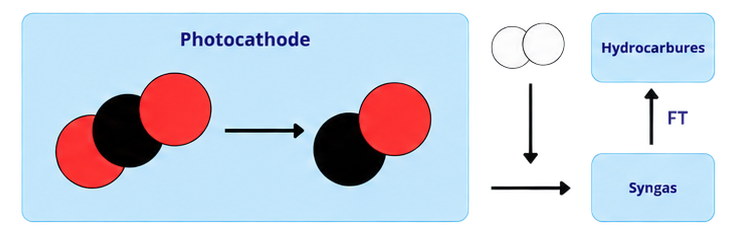
\includegraphics[width=0.98\linewidth]{schema_contexte.png}
        \end{pcbanner}}
    \column{0.42\textwidth}
      \onslide<4->{%
        \begin{pcbanner}{Projet ANR GASPER}
          \vspace{0.25em}
          \begin{itemize}\footnotesize
            \item Réduire le \ch{CO2} en \ch{CO} à l'aide d'une photocathode
            \item 6 laboratoires impliqués
            \item Élaboration, caractérisation et tests des photoélectrodes
            \item Objectifs : efficacité et sélectivité
          \end{itemize}
          \vspace{0.25em}
        \end{pcbanner}}
  \end{columns}
\end{frame}
%==================================================================================================================
%============================================= Fin Contexte =======================================================
%==================================================================================================================

%==================================================================================================================
%===================================== Présentation de la photocathode ============================================
%==================================================================================================================

\section{Présentation de la photocathode}

\begin{frame}[t]{Présentation de la photocathode}

  \vspace{0.3em}

  \begin{columns}[T,onlytextwidth]

    % ------------------ Colonne gauche ------------------
    \column{0.54\textwidth}

      \begin{pcbanner}{Réactions mises en jeu}
        \footnotesize
        \vspace{0.4em}
        \textbf{\color{pcNavy!70}Anode}\\[0.3em]
        \centerline{\normalsize\ch{H2O -> 2 H+ + 2 e- + 1/2 O2}}\\[0.9em]
        \textbf{\color{pcNavy}Cathode}\\[0.3em]
        \centerline{\normalsize\ch{CO2 + 2 H+ + 2 e- -> CO + H2O}}
      \end{pcbanner}

      \vspace{0.4em}

      \begin{pcbanner}{Principe}
        \begin{itemize}\footnotesize
          \item Deux parties : photovoltaïque + électrochimique
          \item Soleil $\rightarrow$ Séparation des charges (partie PV)
          \item Electrons $\rightarrow$ Réduction du \ch{CO2} (partie électrochimique)
        \end{itemize}
      \end{pcbanner}

    % ------------------ Colonne droite ------------------
    \column{0.55\textwidth}

      \centering

      \hspace*{-0.75cm}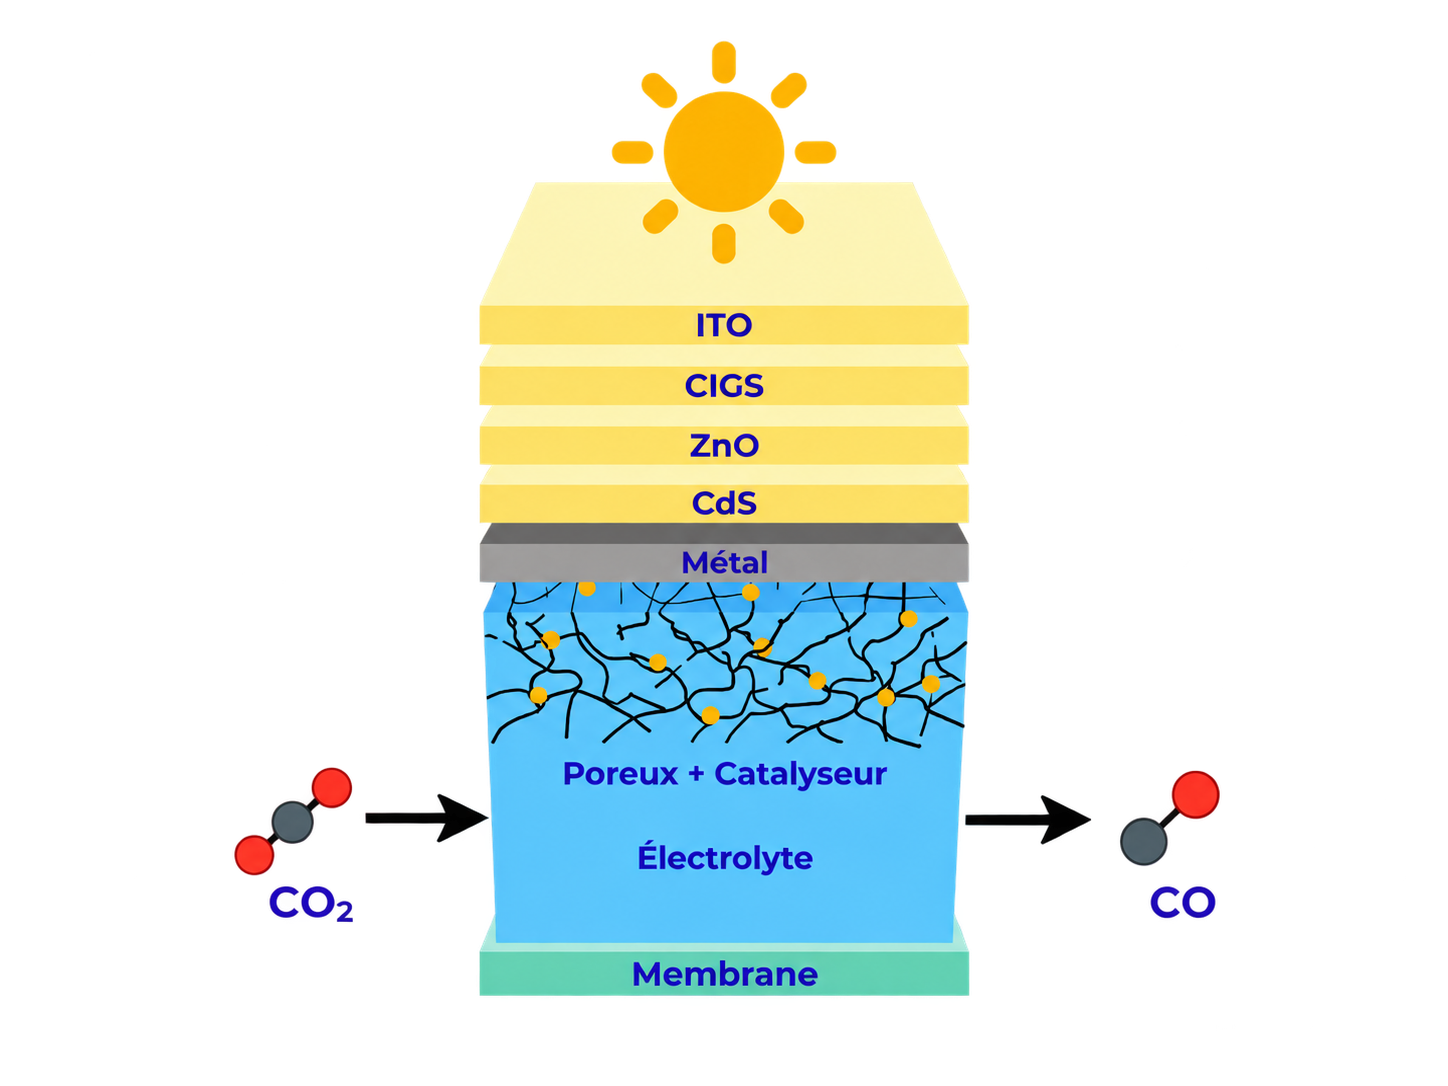
\includegraphics[
        width=1.2\linewidth
      ]{photocathode.png}

  \end{columns}

\end{frame}

%==================================================================================================================
%============================================= Fin Photocathode ===================================================
%==================================================================================================================

%==================================================================================================================
%==================================================== Objectifs ===================================================
%==================================================================================================================
\section{Objectifs}

\begin{frame}[t]{Objectifs}

  \vspace{-0.75em}

  \begin{pcbanner}{Ma contribution dans GASPER}
    \centering
    \footnotesize
      Les partenaires réalisent l'élaboration, la caractérisation et les tests des dispositifs ;
  ma thèse porte sur la \textbf{modélisation de la photocathode}.
  \end{pcbanner}

  \vspace{-0.5em}

  \begin{pcbanner}{Démarche de modélisation}
    \centering
    \figschemademarchemodelo\\[0.5em]
    \vspace{0.5em}
    \footnotesize
    \textcolor{pcNavy}{
      Partie photovoltaïque
      \hspace{1em}+\hspace{1em}
      Partie électrochimique
      \hspace{1em}$\rightarrow$\hspace{1em}
      modèle complet
    }\\
    \textcolor{pcNavy}{(en parallèle : approche par bilan détaillé, transverse aux deux parties)}

  \end{pcbanner}

  \vspace{-0.65em}

\begin{pcbanner}{Finalité}
  \centering
  \footnotesize
  Utiliser le modèle pour guider la montée en échelle (extrapolation), la conception de photocathodes
  plus performantes et permettre ainsi de limiter les essais expérimentaux.
  
\end{pcbanner}

\end{frame}

%==================================================================================================================
%============================================= Fin Objectifs ===================================================
%==================================================================================================================

\section{Modèles}
  % -------------------------------------- Modèles : Partie photovoltaïque ------------------------------------------
\begin{frame}[t]{Modèles : partie photovoltaïque}

  \vspace{-1em}

  \begin{columns}[T,onlytextwidth]

    % ----------- Schéma -----------
    \column{0.48\textwidth}
\begin{pccard}
  \centering
  \figschemaphotovoltaique
  {\scriptsize\bfseries\color{pcNavy}
   Représentation de la partie photovoltaïque}
\end{pccard}


\begin{pcbanner}{Démarche}
  \begin{itemize}\footnotesize
    \item Résolution 1D du système couplé
    \item Comparer aux résultats de SCAPS-1D
    \item Confronter à l'expérimental (ANR)
  \end{itemize}
\end{pcbanner}

    % ----------- Approches -----------
    
        \column{0.48\textwidth}
\vspace{-0.5em}
\begin{pcbanner}{Approche cinétique}
  \vspace{0.45em}
  \begin{pcbannerlight}{Principe}
    \vspace{0.3em}
    \begin{itemize}\footnotesize
      \item Suivi local des porteurs et du potentiel électrostatique
      \item Poisson + équations de continuité
      \item Transport par dérive--diffusion
    \end{itemize}
  \end{pcbannerlight}

  \vspace{0.35em}

  \begin{pcbannerlight}{Physique prise en compte}
    \vspace{0.3em}
    \begin{itemize}\footnotesize
      \item Photogénération (électromagnétisme ou radiatif)
      \item Recombinaisons : SRH, Auger, radiative
      \item Hétérojonction CIGS/CdS/ZnO
    \end{itemize}
  \end{pcbannerlight}
  \vspace{0.2em}
\end{pcbanner}

  \end{columns}


\end{frame}

%------------------------------------------------------------------------

\begin{frame}[t]{Modèles : partie photovoltaïque}

  \vspace{-1em}

  \begin{columns}[T,onlytextwidth]

    % ----------- Schéma -----------
    \column{0.48\textwidth}
\begin{pccard}
  \centering
  \figschemaphotovoltaique

  {\scriptsize\bfseries\color{pcNavy}
   Représentation de la partie photovoltaïque}
\end{pccard}


\begin{pcbanner}{Photogénération}
      \centering\scriptsize
      \textbf{Photogénération (Bouguer--Lambert--Beer)}
      \[ G(x) = q_0\,k_a\,e^{-k_a x} \]
      \end{pcbanner}

    % ----------- Approches -----------
    
    \column{0.48\textwidth}
\vspace{-0.5em}
    \begin{pcbanner}{Système de Van Roosbroeck}
      \vspace{0.3em}
      \centering\scriptsize

      \textbf{Équation de Poisson}
      \[ -\nabla\!\cdot\!\left(\varepsilon\,\nabla\psi\right) = q\,(C + p - n) \]\\

\vspace{1em}
      \textbf{Équations de continuité}
      \[ \frac{\partial n}{\partial t} = \frac{1}{q}\,\nabla\!\cdot\!\vec{J}_n - R + G_{th} + G_{ph} \]
      \[ \frac{\partial p}{\partial t} = -\frac{1}{q}\,\nabla\!\cdot\!\vec{J}_p - R + G_{th} + G_{ph} \]\\

\vspace{1em}
      \textbf{Densités de courant (dérive-diffusion)}
      \[ \vec{J}_n = q\,\mu_n\!\left(-n\,\nabla\psi + U_t\,\nabla n\right) \]
      \[ \vec{J}_p = q\,\mu_p\!\left(-p\,\nabla\psi - U_t\,\nabla p\right) \]\\
\vspace{1em}
      \textbf{CL Robin ou Ohmique}
       \vspace{-0.5em}
    \end{pcbanner}

  \end{columns}


\end{frame}
  % -------------------------------------- Modèles : Partie électrochimique -----------------------------------------

\begin{frame}[t]{Modèles : partie électrochimique}
  \vspace{-1em}

  \begin{columns}[T,onlytextwidth]

    % ----------- Schéma -----------
    \column{0.48\textwidth}
      \begin{pccard}
        \centering
        \figschemaelectrochimique
        \vspace{0.5em}
        {\scriptsize\bfseries\color{pcNavy}
        Représentation de la partie électrochimique}
      \end{pccard}

    % ----------- Différents angles d'approche -----------
    \column{0.48\textwidth}
      \vspace{-0.5em}
      \begin{pcbanner}{Différents angles d'approche}

        %\vspace{-0.25em}

        \begin{pcbannerlight}{Apport du CO2}
          \vspace{0.3em}
          \begin{itemize}\footnotesize
                \item Bullage dans l'électrolyte 
                \item Electrode à diffusion de gaz (GDE)
          \end{itemize}
        \end{pcbannerlight}

        \vspace{-0.5em}

        \begin{pcbannerlight}{Géométrie de l'électrode}
          \vspace{0.3em}
          \begin{itemize}\footnotesize
            \item Modèle 3D local 
            \item Modèle 1D macroscopique
          \end{itemize}
        \end{pcbannerlight}

      \end{pcbanner}
    \end{columns}


    \vspace{-0.75em}
    \begin{columns}[T,onlytextwidth]
      \column{\textwidth}
        \begin{pcbanner}{Démarche}
          \begin{itemize}\footnotesize
            \item Comparer 1D et 3D (homogénéisation)
            \item Comparer les deux configurations (électrode à diffusion de gaz / bullage dans l'électrolyte)
            \item Confronter à l'expérimental (partenaires GASPER)
          \end{itemize}
        \end{pcbanner}
    \end{columns}

\end{frame}


%--------------------------------------------------------------------
\begin{frame}[t]{Modèles : partie électrochimique}
  \vspace{-1em}

  \begin{columns}[T,onlytextwidth]

    % ----------- Schéma (inchangé) -----------
     \column{0.48\textwidth}
      \begin{pccard}
        \centering
        \figschemaelectrochimique
        \begin{tikzpicture}[remember picture, overlay]
          \draw[pcSun, line width=1.5pt]
            ([xshift=-4.35cm, yshift=0.91cm]current page.center)
            ellipse [x radius=0.6cm, y radius=1.1cm];
        \end{tikzpicture}
        \vspace{0.5em}
        {\scriptsize\bfseries\color{pcNavy}
        Représentation de la partie électrochimique}
      \end{pccard}

      \begin{pcbanner}{Réduction du \ch{CO2}}
      \centering\scriptsize
      \textbf{Équation de réaction}
      \[ \mathrm{CO_2} + 2\,\mathrm{H^+} + 2\,\mathrm{e^-} \rightarrow \mathrm{CO} + \mathrm{H_2O} \]
      \end{pcbanner}

    % ----------- Modèle électrochimique -----------
    \column{0.48\textwidth}
      \vspace{-0.5em}
        \begin{pcbanner}{Modèle dans le milieu poreux}
        \vspace{0.4em}
        \centering\scriptsize
        \textbf{Équation de conservation}
        \[ \frac{\partial C_i}{\partial t} + \nabla\!\cdot\! N_i = 0 \]
        \textbf{Transport des espèces (Nernst--Planck)}
        \[ N_i = -D_i\nabla C_i - \frac{z_i F}{RT}\,D_i C_i\,\nabla\varphi_l + C_i\,\vec{v} \]

        \textbf{Électroneutralité} \qquad \textbf{Transport électronique (Ohm)}
        \[ \sum_i z_i C_i = 0 \qquad \qquad \qquad \nabla\!\cdot\!\left(-\sigma_s\,\nabla\varphi_s\right) = 0 \]

        \textbf{Cinétique interfaciale}\\[0.3em]
        \begin{itemize}\scriptsize
          \item Butler--Volmer (semi-empirique)
          \item Marcus--Gerischer (théorique)
        \end{itemize}
        \end{pcbanner}

    \end{columns}

\end{frame}

%--------------------------------------------------------------------
\begin{frame}[t]{Electrochimie : cas simplifié \ch{CO2} -> \ch{CO}}
  \vspace{-1em}

  \begin{columns}[T,onlytextwidth]

    % ----------- Colonne gauche : hypothèses -----------
      \column{0.48\textwidth}
\vspace{-0.5em}

   \begin{pcbanner}{Module de Thiele $\phi$}
        \footnotesize
        Compétition diffusion / réaction :
        \begin{itemize}\footnotesize
        \item $\phi \ll 1$ : diffusion rapide $\rightarrow$ concentration uniforme
        \item $\phi \gg 1$ : réaction rapide $\rightarrow$ \ch{CO2} consommé près de l'interface
        \end{itemize}
      \end{pcbanner}

      \begin{pcbanner}{Hypothèses (approche de Thiele)}
        \vspace{0.15em}
        \begin{itemize}\footnotesize
          \item Régime stationnaire, transport purement diffusif
          \item Migration, convection, chute ohmique négligées
          \item Deux espèces carbonées seulement : \ch{CO2}, \ch{CO}
          \item Réaction globale simplifiée \ch{CO2 -> CO}
        \end{itemize}
      \end{pcbanner}

    % ----------- Colonne droite : modèle + solution -----------
    \column{0.48\textwidth}
      \vspace{-0.5em}
      \begin{pcbanner}{Système diffusion--réaction}
        \centering\scriptsize
       \textbf{Forme adimensionnée (module de Thiele $\phi$)}
        \[ \frac{\mathrm{d}^2 \langle C_{\ch{CO2}}\rangle^l}{\mathrm{d}\zeta^2}
           = \phi^2\, \langle C_{\ch{CO2}}\rangle^l \]
        \[ \frac{\mathrm{d}^2 \langle C_{\ch{CO}}\rangle^l}{\mathrm{d}\zeta^2}
           = -\,\frac{a_v^{\mathrm{cat}}\, k\, l_e^2}{\varepsilon_l D^{\mathrm{eff}}_{\ch{CO}}}
             \, \langle C_{\ch{CO2}}\rangle^l \]
      \end{pcbanner}

      \begin{pcbanner}{Solution analytique}
        \vspace{-0.5em}
        \centering\scriptsize
        \[ \langle C_{\ch{CO2}}\rangle_l(\zeta)
           = C^{\mathrm{hom}}_{\ch{CO2}}\,
             \frac{\cosh[\phi(\zeta+1)]}{\cosh(\phi)} \]
        \[ \langle C_{\ch{CO}}\rangle_l(\zeta)
           = C^{\mathrm{hom}}_{\ch{CO}}
           + \frac{D^{\mathrm{eff}}_{\ch{CO2}}}{D^{\mathrm{eff}}_{\ch{CO}}}
             \,C^{\mathrm{hom}}_{\ch{CO2}}
             \left[1 - \frac{\cosh[\phi(\zeta+1)]}{\cosh(\phi)}\right] \]
      \end{pcbanner}

    \end{columns}

\end{frame}
\section{Bilan sur la première année}
  % --------------------------------------- Bilan : Brique photovoltaïque -------------------------------------------

\begin{frame}[t]{Bilan : brique photovoltaïque}
  \vspace{0.3em}
  \begin{columns}[T,onlytextwidth]
    \column{0.48\textwidth}
      \begin{pcbanner}{Avancées}
        \begin{itemize}\footnotesize
          \item Solveur 1D en C : Poisson + deux continuités
          \item Génération Bouger
          \item Recombinaisons SRH, Auger, radiatif
          \item Recherche sur l'hétérojonction CIGS/CdS/ZnO
          \item Recherche sur des CL plus réalistes
        \end{itemize}
      \end{pcbanner}
    \column{0.48\textwidth}
      \begin{pcbanner}{Jalons clés}
        \begin{itemize}\footnotesize
          \item 1\textsuperscript{re} version : Newton stationnaire, adimensionnée
          \item Comparaison sans génération réussi avec Farrell \textit{et al.}
          \item Blocage à la photogénération
          \item Levé par passage en résolution transitoire
          \item Comparaison réussi pour l'homojonction et CL ohmique avec et sans génération
        \end{itemize}
      \end{pcbanner}
  \end{columns}

  \vspace{0.3em}
  \begin{columns}[T,onlytextwidth]
    \column{\textwidth}
      \begin{pcbanner}{Validation}
        \begin{itemize}\footnotesize
          \item Cas sans génération : accord avec Farrell \textit{et al.}
          \item Cas avec génération (ohmique et homojonctions) : accord avec SCAPS 1D 
        \end{itemize}
      \end{pcbanner}
  \end{columns}
\end{frame}

 \begin{frame}[t]{Brique photovoltaïque : validation}
   \vspace{-0.5em}
   \centering
   \begin{pccard}
     \centering
     \begin{tikzpicture}
      \begin{axis}[
        width=0.9\linewidth, height=0.72\textheight,
        xlabel={$x$ ($\mu$m)},
        ylabel={Densités de porteurs ($\mathrm{m^{-3}}$)},
        ymode=log,
        legend pos=outer north east,
        legend style={font=\scriptsize, cells={anchor=west}},
        grid=both, grid style={gray!20},
        tick label style={font=\scriptsize},
        label style={font=\scriptsize},
      ]
        % --- Électrons n ---
         \addplot[pcNavy, only marks, mark=o, mark size=1.1pt, each nth point=4]
                 table[x=x, y=n_scaps, col sep=semicolon] {donnees1.csv};
         \addlegendentry{$n$ (code)}
         \addplot[pcNavy, thick] table[x=x, y=n_code, col sep=semicolon] {donnees1.csv};
         \addlegendentry{$n$ (SCAPS)}
        % % --- Trous p ---
        \addplot[pcSunDeep, only marks, mark=square, mark size=1.1pt, each nth point=4]
                 table[x=x, y=p_scaps, col sep=semicolon] {donnees1.csv};
        \addlegendentry{$p$ (code)}
        \addplot[pcSunDeep, thick] table[x=x, y=p_code, col sep=semicolon] {donnees1.csv};
        \addlegendentry{$p$ (SCAPS)}
        \end{axis}
     \end{tikzpicture}

     {\scriptsize\bfseries\color{pcNavy}
      Densités de porteurs en fonction de la position : comparaison code / SCAPS-1D pour CIGS dopé n/CIGS dopé p avec photogénération}
   \end{pccard}
 \end{frame}

  % --------------------------------------- Bilan : Brique électrochimique -------------------------------------------

\begin{frame}[t]{Bilan : brique électrochimique}
  \vspace{0.3em}
  \begin{columns}[T,onlytextwidth]
    \column{\textwidth}
      \begin{pcbanner}{Avancées}
        \begin{itemize}\footnotesize
          \item Modèle 3D local : Nernst--Planck, loi d'Ohm, Marcus--Gerischer
          \item Réduction 1D par homogénéisation (coefficients effectifs)
          \item Modèle de Thiele en cas limite (facteur d'efficacité)
          \item Réaction globale simplifiée \ch{CO2 -> CO} 
          \item Étude bibliographique (lois de vitesse)
          \item Revue des phénomènes influençant l'électrode
        \end{itemize}
      \end{pcbanner}
  \end{columns}

  \vspace{0.3em}
  \begin{columns}[T,onlytextwidth]
    \column{\textwidth}
      \begin{pcbanner}{Validation}
        \begin{itemize}\footnotesize
          \item Implémentation et validation prévues en année 2
        \end{itemize}
      \end{pcbanner}
  \end{columns}
\end{frame}
%==================================================================================================================
%================================================ Perspectives ====================================================
%==================================================================================================================

% --------------------------------- Perspectives : Complémenter et construire -------------------------------------
\section{Perspectives}
\begin{frame}[t]{Perspectives : compléter et construire}
  \vspace{0.4em}

  \begin{columns}[T,onlytextwidth]
    \column{0.48\textwidth}
      \begin{pcbanner}{Brique photovoltaïque}
        \begin{itemize}\footnotesize
          \item Ajouter les hétérojonctions
          \item Revoir les conditions aux limites
          \item Compléter la partie optique 
          \item Valider sur les données de l'ANR
          \item Intégrer des phénomènes fins si nécessaire
        \end{itemize}
      \end{pcbanner}
    \column{0.48\textwidth}
      \begin{pcbanner}{Brique Electrochimique}
        \begin{itemize}\footnotesize
          \item Partie hors du milieu poreux 
          \item Modèle GDE
          \item Vérifier la loi de vitesse (données ANR)
          \item Valider sur les données de l'ANR
          \item Intégrer des phénomènes fins si nécessaire (HER, pH, double couche\dots)
        \end{itemize}
      \end{pcbanner}
  \end{columns}

  \vspace{0.35em}
  \begin{columns}[T,onlytextwidth]
    \column{\textwidth}
      \begin{pcbanner}{Construire/Comprendre de nouvelles briques}
        \begin{itemize}\footnotesize
          \item Phototgénération : passer à l'electromagnétique
          \item \textit{Detailed balance} : approche alternative 
        \end{itemize}
      \end{pcbanner}
  \end{columns}
\end{frame}

% ---------------------------------- Perspectives : Coupler et optimiser -------------------------------------
\begin{frame}[t]{Perspectives : coupler et optimiser}
  \vspace{0.4em}

  \begin{pcbanner}{Coupler les briques}
    \begin{itemize}\footnotesize
      \item Articuler les briques une fois complétées et validées (notamment les CL)
      \item Commencer par l'interface semi-conducteur / électrolyte
    \end{itemize}
  \end{pcbanner}

  \vspace{0.8em}

  \begin{pcbanner}{Objectif final : Outil d'analyse d'extrapolation et d'optimisation}
    \begin{itemize}\footnotesize
      \item Modèle couplé et prédictif $\rightarrow$ explorer l'espace des géométries
      \item Épaisseurs, structure poreuse, aire catalytique
      \item Maximiser le courant et le rendement de production de \ch{CO}
    \end{itemize}
  \end{pcbanner}
\end{frame}


%==================================================================================================================
%================================================ Fin Perspectives ================================================
%==================================================================================================================

\section{Formations}

\begin{frame}[t]{Formations suivies}

  \vspace{-0.5em}

  \begin{columns}[T,onlytextwidth]

    \column{0.48\textwidth}
      \begin{pcbanner}{Formations scientifiques}
        \begin{itemize}\footnotesize
          \item Ecole de physique des Houches
          \item Séminaire Monte Carlo Roffiac
        \end{itemize}
      \end{pcbanner}

      \begin{pcbanner}{Formations transversales}
        \begin{itemize}\footnotesize
          \item Festival les nuées ardentes
          \item Journée Scientifique SPI
        \end{itemize}
      \end{pcbanner}

  
  \column{0.48\textwidth}

  \begin{center}
    \setlength{\fboxrule}{1pt}
    \setlength{\fboxsep}{0pt}
    \fcolorbox{pcNavy}{white}{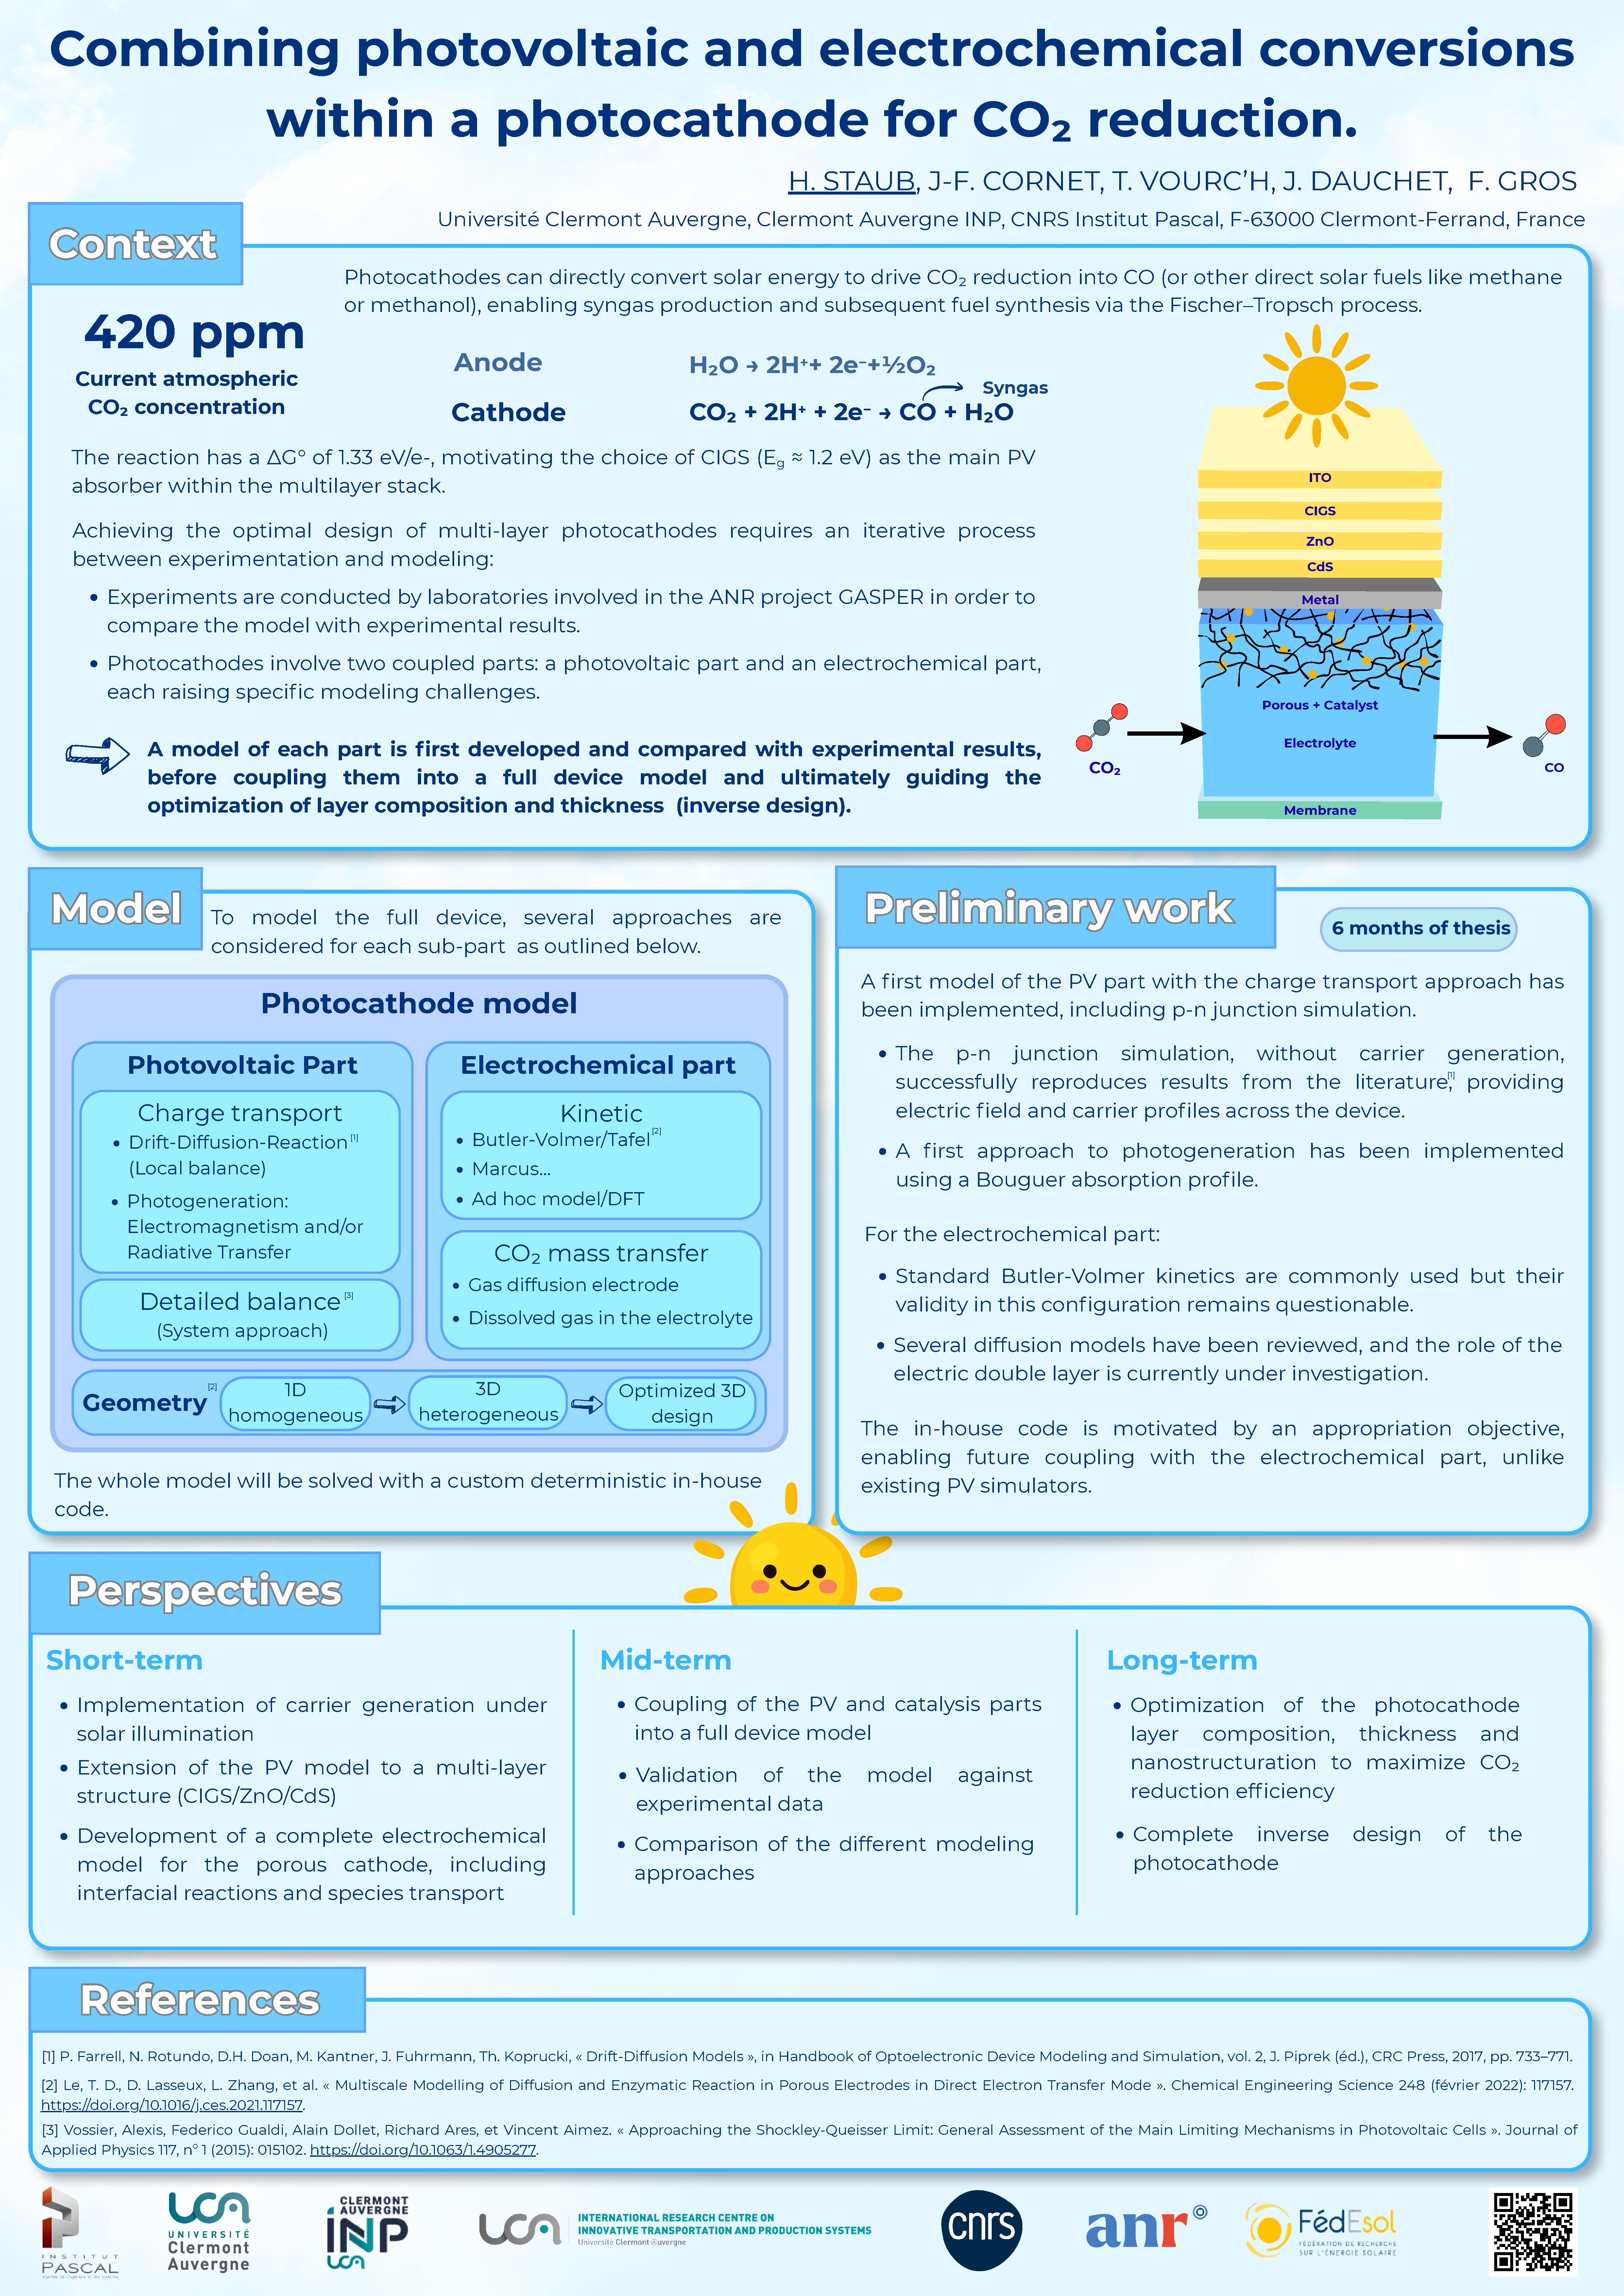
\includegraphics[page=1,height=0.75\textheight]{poster.pdf}}
  \end{center}
\end{columns}

\end{frame}
% ====================================================================
% ====================================================================
% ====================================================================
%  Frame Gantt (échelle en MOIS) — Calendrier prévisionnel de la thèse
%  PRÉREQUIS dans le préambule :  \usepackage{pgfgantt}
%
%  Chaque case = 1 mois. L'axe démarre en NOVEMBRE 2025 (mois 1) et
%  couvre 36 mois (nov 2025 -> oct 2028). La 1re ligne = année de thèse
%  (nov->oct), la 2e = initiale du mois (N D J F M A M J J A S O).
%  Le trait pointillé orange = position actuelle (~ sept 2026, mois 11).
%  NB : les nombres des \ganttbar sont des indices de mois, 1 = nov 2025.
% ====================================================================

\section{Gantt : calendrier prévisionnel}
\begin{frame}[t]{Calendrier prévisionnel}

  \vspace{-2em}
  \begin{pccard}
    % Cale le graphe à gauche (au lieu de le centrer) : la marge négative
    % remonte les intitulés vers le bord gauche. Ajuste -1.2cm si besoin.
    \noindent\hspace*{-0.55cm}%
        \begin{ganttchart}[
        x unit=0.7cm,
        hgrid, vgrid={*3{draw=gray!12}, *1{draw=gray!25}},
        canvas/.style={draw=gray!40, line width=.5pt},
        y unit title=0.38cm, y unit chart=0.38cm,
        title height=1, title/.style={fill=none},
        title label font=\tiny\bfseries\color{pcNavy},
        group label font=\scriptsize\bfseries\color{pcNavy},
        bar label font=\scriptsize\color{pcNavy!80},
        group label node/.append style={left=0.15cm},
        bar label node/.append style={left=0.4cm},
        group/.append style={draw=none, fill=pcNavy!70},
        group height=.5, group peaks tip position=0,
        bar/.append style={draw=none, fill=pcBlue!75}, bar height=.6,
      ]{1}{12}

      % --- Bandeau 1 : année de thèse ---
      \gantttitle{Année 1 (2025--26)}{4}
      \gantttitle{Année 2 (2026--27)}{4}
      \gantttitle{Année 3 (2027--28)}{4}                       \\
      % --- Bandeau 2 : trimestres ---
      \gantttitle{T1}{1}\gantttitle{T2}{1}\gantttitle{T3}{1}\gantttitle{T4}{1}%
      \gantttitle{T1}{1}\gantttitle{T2}{1}\gantttitle{T3}{1}\gantttitle{T4}{1}%
      \gantttitle{T1}{1}\gantttitle{T2}{1}\gantttitle{T3}{1}\gantttitle{T4}{1} \\

      % ---------- Brique photovoltaïque ----------
      \ganttgroup{Semi-conducteur}{1}{7}                       \\
      \ganttbar{Solveur 1D (Van Roosbroeck)}{1}{7}             \\
      \ganttbar{Validation (Farrell, SCAPS)}{3}{7}             \\
      \ganttbar[bar/.append style={fill=pcSun!70}]%
               {Hétérojonctions \& CL de Robin}{5}{6}          \\
      \ganttbar[bar/.append style={fill=pcSun!70}]%
               {Validation données ANR}{7}{9}                  \\

      % ---------- Brique électrochimique ----------
      \ganttgroup{Électrochimie}{2}{9}                         \\
      \ganttbar{Modèle 3D $\rightarrow$ 1D (homogénéisation)}{2}{4} \\
      \ganttbar[bar/.append style={fill=pcSun!70}]%
               {Implémentation + modèle GDE}{5}{8}             \\
      \ganttbar[bar/.append style={fill=pcSun!70}]%
               {Validation données ANR}{8}{9}                  \\

      % ---------- Nouvelles briques ----------
      \ganttgroup{Nouvelles briques}{5}{8}                     \\
      \ganttbar[bar/.append style={fill=pcSun!70}]%
               {Photogénération}{5}{8}  \\
      \ganttbar[bar/.append style={fill=pcSun!70}]%
               {\textit{Detailed balance}}{7}{9}               \\

      % ---------- Couplage & optimisation ----------
      \ganttgroup{Couplage \& optimisation}{9}{12}             \\
      \ganttbar[bar/.append style={fill=pcSun!70}]%
               {Couplage des briques}{9}{11}                   \\
      \ganttbar[bar/.append style={fill=pcSun!70}]%
               {Outil d'optimisation}{10}{12}                  \\

      % ---------- Rédaction ----------
      \ganttbar[bar/.append style={fill=pcNavy!55}]%
               {Rédaction \& soutenance}{10}{12}               \\

      % ---------- Ligne "aujourd'hui" (~ sept. 2026, milieu du T4 année 1) ----------
      \ganttvrule[vrule/.style={pcSunDeep, line width=1pt, dashed},
                  vrule offset=0.5]%
                 {}{4}

    \end{ganttchart}

    \vspace{0.2em}
    \centering
    {\scriptsize\bfseries\color{pcNavy}
     Planning prévisionnel sur les trois années de thèse — %
     \textcolor{pcBlue!75}{$\blacksquare$}~réalisé \quad
     \textcolor{pcSun!70!black}{$\blacksquare$}~à venir \quad
     \textcolor{pcSunDeep}{$\dashv$}~aujourd'hui}
  \end{pccard}

\end{frame}

%==================================================================================================================
%======================================== Fin Insertion des diapos ================================================
%==================================================================================================================
%------------------------------------------------------------------------------------------------------------------

%==================================================================================================================
%========================================================= Fin ====================================================
%==================================================================================================================

{\setbeamertemplate{footline}{}
\begin{frame}[plain]
  \centering
  \vspace{5em}
  {\Huge\bfseries\color{pcNavy}Merci de votre attention}\\[0.4cm]
  {\color{pcBlue}Avez vous des questions ?}
    \begin{tikzpicture}[remember picture,overlay]
    \node[anchor=south east] at ($(current page.south east)+(-1,1)$)
      {
\includegraphics[width=4.5cm]{soleil.png}};
  \end{tikzpicture}%
\end{frame}}




\appendix
%==================================================================================================================
%==================================================== Différentes recombinaisons =======================================================
%==================================================================================================================

\begin{frame}[t]{Différentes types de recombinaisons}
  \vspace{-0.5em}
  \centering
      \begin{pccard}
        \centering
        \figrecombinaison
        \vspace{0.5em}
        {\scriptsize\bfseries\color{pcNavy}
        Différents types de recombinaisons : SRH, radiative et Auger}
      \end{pccard}
\end{frame}

%------------------------------------------------------------------------------------------------------------------

\begin{frame}[t]{Annexe : conditions aux limites — semi-conducteur}
  \vspace{-0.5em}

  \begin{columns}[T,onlytextwidth]

    \column{0.48\textwidth}
      \begin{pcbanner}{Contacts ohmiques (retenu)}
        \centering\scriptsize
        \textbf{Poisson : Dirichlet sur le potentiel}
        \[ \psi = \psi_0 + U_{\mathrm{app}} \]
        {\raggedright tension appliquée répartie symétriquement sur les deux contacts\par}
        \vspace{0.4em}
        \textbf{Densités : valeurs d'équilibre figées}
        \[ n = n_{\mathrm{eq}}, \qquad p = p_{\mathrm{eq}} \]
        {\raggedright nœuds de bord non mis à jour par le schéma temporel\par}
      \end{pcbanner}

    \column{0.48\textwidth}
      \begin{pcbanner}{Recombinaison de surface finie (perspective)}
        \begin{itemize}\footnotesize
          \item Hypothèse actuelle : contacts ohmiques idéaux (forte)
          \item Alternative : conditions de \textbf{Robin}
          \item Permet une recombinaison de surface finie aux contacts
          \item Objet de comparaison à venir
        \end{itemize}
      \end{pcbanner}

  \end{columns}

\end{frame}
%----------------------------------------------------------------------------------------

\begin{frame}[t]{Modèle 1D homogénéisé}
  \vspace{-0.5em}

  \begin{columns}[T,onlytextwidth]

    \column{0.46\textwidth}
      \begin{pccard}
        \centering
        \figschemaelectrochimique
        \vspace{0.4em}
        {\scriptsize\bfseries\color{pcNavy}
        Prise de moyenne volumique : 3D pore $\rightarrow$ 1D électrode}
      \end{pccard}

      \begin{pcbanner}{Principe}
        \begin{itemize}\footnotesize
          \item Moyenne sur un volume élémentaire représentatif
          \item Microstructure incorporée dans des coefficients effectifs
          \item Fermeture par vecteurs $b$, $d$, $e$
        \end{itemize}
      \end{pcbanner}

    \column{0.52\textwidth}
      \vspace{-0.5em}
      \begin{pcbanner}{Système homogénéisé}
        \centering\scriptsize
        \textbf{Conservation des espèces}
        \[ \varepsilon_l\frac{\partial \langle C_i\rangle^l}{\partial t}
           = \nabla\!\cdot\!\Big[ D_i^{\mathrm{tot}}\nabla\langle C_i\rangle^l
           + \tfrac{z_i F}{RT}\varepsilon_l D_i^{\mathrm{eff,mig}}
             \langle C_i\rangle^l \nabla\langle\varphi_l\rangle^l
           - \varepsilon_l \langle C_i\rangle^l \langle v\rangle^l \Big]
           + a_v^{\mathrm{cat}} R_i \]

        \textbf{Électroneutralité}
        \[ \sum_i z_i \langle C_i\rangle^l = 0 \]

        \textbf{Loi d'Ohm (phase solide)}
        \[ \nabla\!\cdot\!\big(\varepsilon_s \sigma^{\mathrm{eff}}
           \nabla\langle\varphi_s\rangle^s\big) = -\,a_v^{\mathrm{cat}}\, j \]

        \vspace{0.3em}
        \textbf{Coefficients effectifs}\\[0.2em]
        $D_i^{\mathrm{tot}} = \varepsilon_l D_i^{\mathrm{eff}} + D^{\mathrm{disp}}$,
        \quad $\sigma^{\mathrm{eff}}$, \quad $a_v^{\mathrm{cat}} = \theta a_v$
      \end{pcbanner}

  \end{columns}

\end{frame}

%----------------------------------------------------------------------------------------

\begin{frame}[t]{Annexe : réduction au module de Thiele}
  \vspace{-0.5em}

  \begin{columns}[T,onlytextwidth]

    \column{0.48\textwidth}
      \begin{pcbanner}{Hypothèses successives}
        \begin{itemize}\footnotesize
          \item Régime stationnaire
          \item Convection négligée ($\langle v\rangle^l = 0$)
          \item Migration négligée
          \item Potentiel solide uniforme ($\nabla\langle\varphi_s\rangle^s = 0$)
          \item Cinétique du 1\textsuperscript{er} ordre (Butler--Volmer linéarisée)
        \end{itemize}
      \end{pcbanner}

    \column{0.48\textwidth}
      \vspace{-0.5em}
      \begin{pcbanner}{Équation de diffusion--réaction}
        \centering\scriptsize
        \[ \frac{\mathrm{d}^2 \langle C_i\rangle^{l,*}}{\mathrm{d}\zeta^2}
           = \phi^2\, \langle C_i\rangle^{l,*} \]

        \textbf{Module de Thiele}
        \[ \phi^2 = -\,\frac{\nu_i\, a_v^{\mathrm{cat}}\, k(\eta)\, l_e^2}
                          {n_e F\, \varepsilon_l D_i^{\mathrm{eff}}} \]

        \textbf{Facteur d'efficacité}
        \[ \eta_E = \frac{\tanh(\phi)}{\phi} \]

        \vspace{0.2em}
        {\raggedright $\phi \ll 1$ : diffusion rapide, concentration uniforme\\
        $\phi \gg 1$ : réaction rapide, chute près de l'interface\par}
      \end{pcbanner}

  \end{columns}

\end{frame}

%--------------------------------------------------------------------------------

\begin{frame}[t]{Annexe : conditions aux limites — électrochimie}
  \vspace{-0.5em}

  \begin{columns}[T,onlytextwidth]

    \column{0.5\textwidth}
      \begin{pcbanner}{Système homogénéisé 1D}
        \centering\scriptsize
        \textbf{Collecteur de courant}
        \[ \langle N_i\rangle^l\!\cdot\!n = 0, \quad
           n\!\cdot\!\nabla\langle\varphi_l\rangle^l = 0, \quad
           \langle\varphi_s\rangle^s = E \]

        \vspace{0.3em}
        \textbf{Interface pore / milieu homogène}
        \[ \langle C_i\rangle^l = C_i^{\mathrm{hom}}, \quad
           \langle\varphi_l\rangle^l = \varphi_l^{\mathrm{hom}} \]
        \[ n\!\cdot\!\big(\varepsilon_s\sigma^{\mathrm{eff}}
           \nabla\langle\varphi_s\rangle^s\big) = 0 \]
      \end{pcbanner}

    \column{0.5\textwidth}
      \vspace{-0.5em}
      \begin{pcbanner}{Cas simplifié \ch{CO2 -> CO}}
        \centering\scriptsize
        \textbf{Concentration imposée au bulk ($\zeta = 0$)}
        \[ \langle C_{\ch{CO2}}\rangle^l(0) = C^{\mathrm{hom}}_{\ch{CO2}}, \quad
           \langle C_{\ch{CO}}\rangle^l(0) = C^{\mathrm{hom}}_{\ch{CO}} \]

        \vspace{0.3em}
        \textbf{Flux nul à la paroi ($\zeta = -1$)}
        \[ \frac{\mathrm{d}\langle C_{\ch{CO2}}\rangle^l}{\mathrm{d}\zeta}(-1) = 0, \quad
           \frac{\mathrm{d}\langle C_{\ch{CO}}\rangle^l}{\mathrm{d}\zeta}(-1) = 0 \]
      \end{pcbanner}

  \end{columns}

\end{frame}

\end{document}